\documentclass[12pt]{article}
\usepackage{graphicx}
\usepackage[margin=1in]{geometry}
\usepackage{tikz}
\usepackage{listings}
\usepackage{color} % Required for custom colors
\usepackage{courier} % Set the font for listing as Courier
% Define custom colors
\definecolor{mygreen}{rgb}{0,0.6,0}
\definecolor{mygray}{rgb}{0.5,0.5,0.5}
\definecolor{mymauve}{rgb}{0.58,0,0.82}

% Define the MATLAB code style
\lstdefinestyle{mystyle}{
    backgroundcolor=\color{white},
    basicstyle=\footnotesize\ttfamily,
    commentstyle=\color{mygreen},
    keywordstyle=\color{blue},
    numberstyle=\tiny\color{mygray},
    numbers=left,
    numbersep=5pt,
    showspaces=false,
    showstringspaces=false,
    showtabs=false,
    tabsize=2,
    fontadjust=true,
    columns=fullflexible,
    keepspaces=true
}
\lstset{style=mystyle}

\begin{document}

\title{ELCT 432: Problem Assignment \#5}
\author{Jacob C. Vaught}
\date{10-28-2023}
\maketitle

\subsection*{Explanation of the Program}
The MATLAB program performs the following tasks:
\begin{itemize}
    \item Generates a random sequence of bits with lengths \(N = 10, 100, 1000, 10^4\).
    \item Calculates the mean, variance, and power of these sequences.
    \item Plots the random sequence for \(N = 10\).
    \item Plots histograms for \(N = 10\) and \(N = 10^4\).
\end{itemize}

\subsubsection*{Random Bit Sequence Plot for \(N = 10\)}
\begin{center} 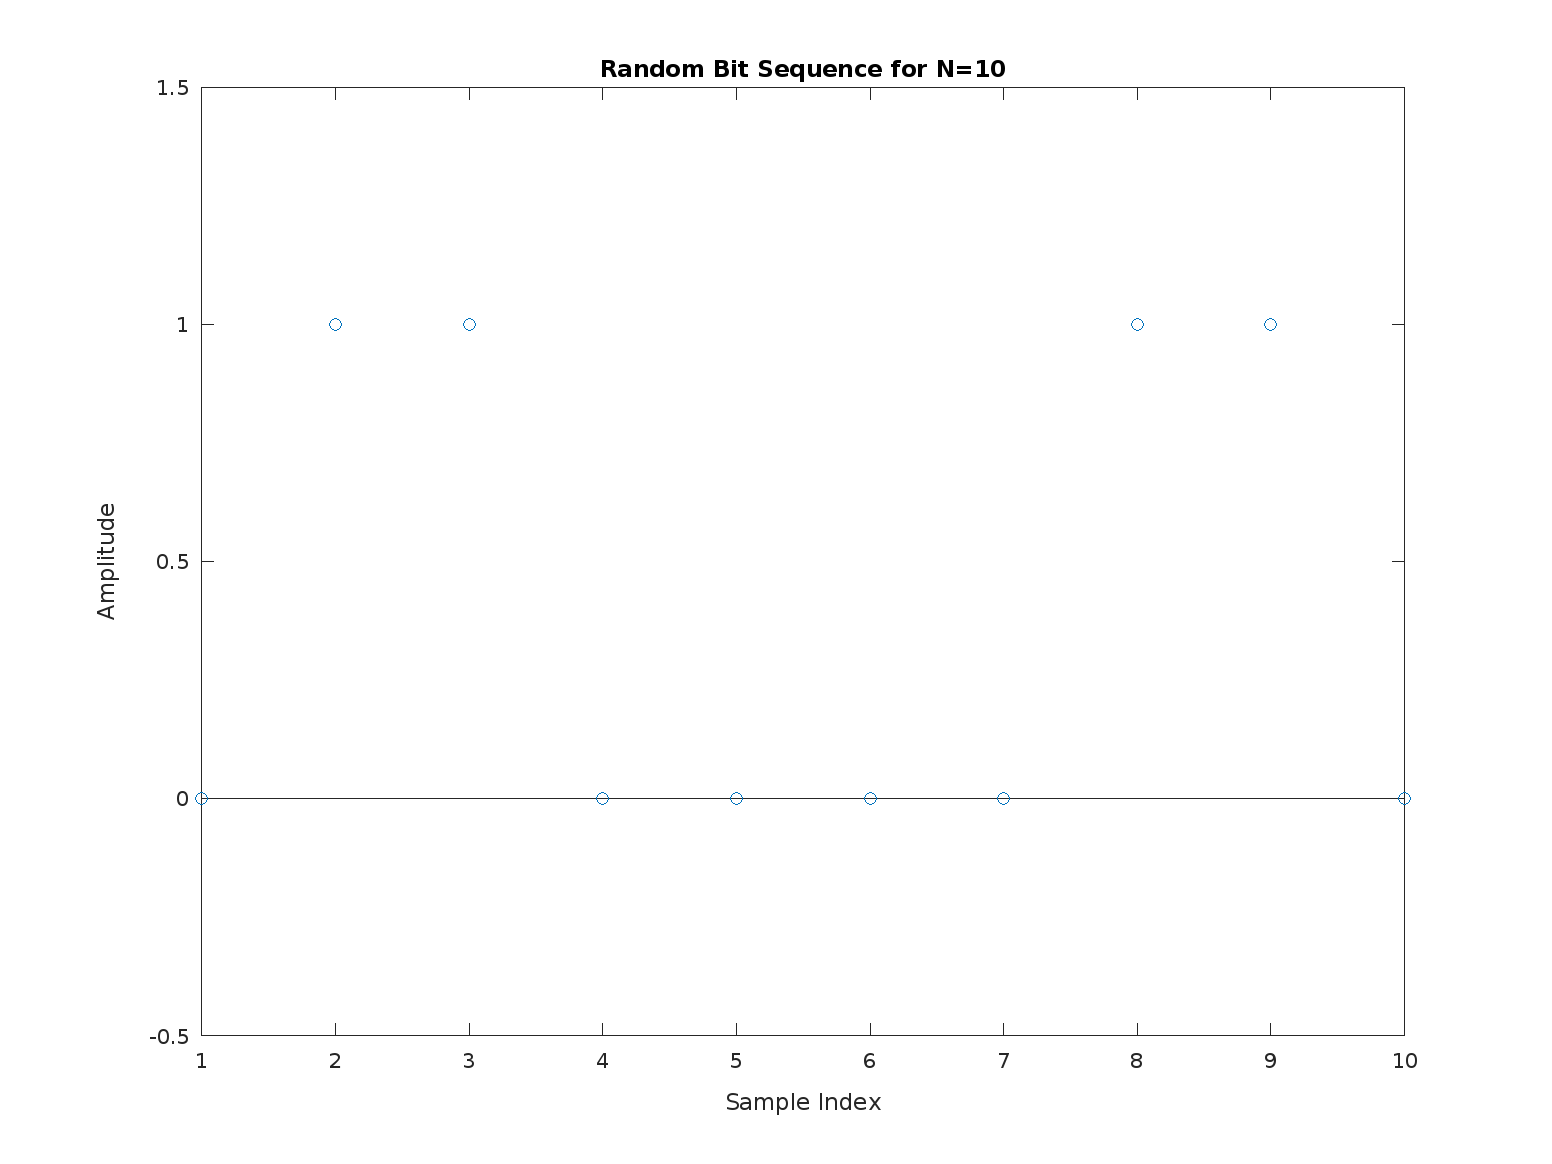
\includegraphics[width=0.8\textwidth]{random_bit_sequence.png}\end{center}

\subsection*{Statistical Analysis}

\begin{itemize}
    \item Expected Mean: The expected mean of a sequence of equiprobable random variables \( \{-1, 1\} \) is \(0\), because \(E[X] = (-1 \times 0.5) + (1 \times 0.5) = 0\).
    
    \item Expected Variance: The expected variance is \(1\), calculated as \( \text{Var}[X] = E[X^2] - (E[X])^2 = 1 - 0^2 = 1 \).
    
    \item Expected Power: Power is the mean of the square of the sequence elements, which is also \(1\), same as the variance in this case.
\end{itemize}

\subsection*{Comparison with MATLAB Results}

\begin{center}
\begin{tabular}{|c|c|c|c|}
\hline
\(N\) & Mean & Variance & Power \\
\hline
10 & 0.8 & 0.4 & 1 \\
100 & -0.04 & 1.0085 & 1 \\
1000 & 0.02 & 1.0006 & 1 \\
10000 & 0.0062 & 1.0001 & 1 \\
\hline
\end{tabular}
\end{center}
\newline\newline
The computed mean, variance, and power values should converge to the theoretical values as \(N\) increases. This is in accordance with the Law of Large Numbers. As observed, for \(N=10\), the results differ more from the theoretical values. However, as \(N\) increases to 10000, the values become very close to the theoretical expectations, which validates the Law of Large Numbers.


\section*{PMF}
\begin{figure}[h!]
  \centering
  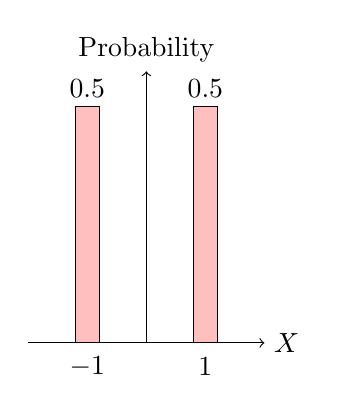
\begin{tikzpicture}[scale=1.5]
    \draw[->] (-1,0) -- (1,0) node[right] {\(X\)};
    \draw[->] (0,0) -- (0,2.3) node[above] {Probability};
    
    \foreach \x/\y in {-1/0.5, 1/0.5} {
      \draw[fill=pink] (\x*0.5-0.1,0) rectangle ++(0.2,\y*4);
      \node at (\x*0.5, \y*4.3) { \(\y\)};
    }
    
    \foreach \x/\y in {-1/-1, 1/1} {
      \node at (\x*0.5, -0.2) { \(\y\)};
    }
  \end{tikzpicture}
  \caption{PMF of Random Variable \(X\)}
\end{figure}

\subsubsection*{Histograms for \(N = 10\) and \(N = 10^4\)}
\begin{center} 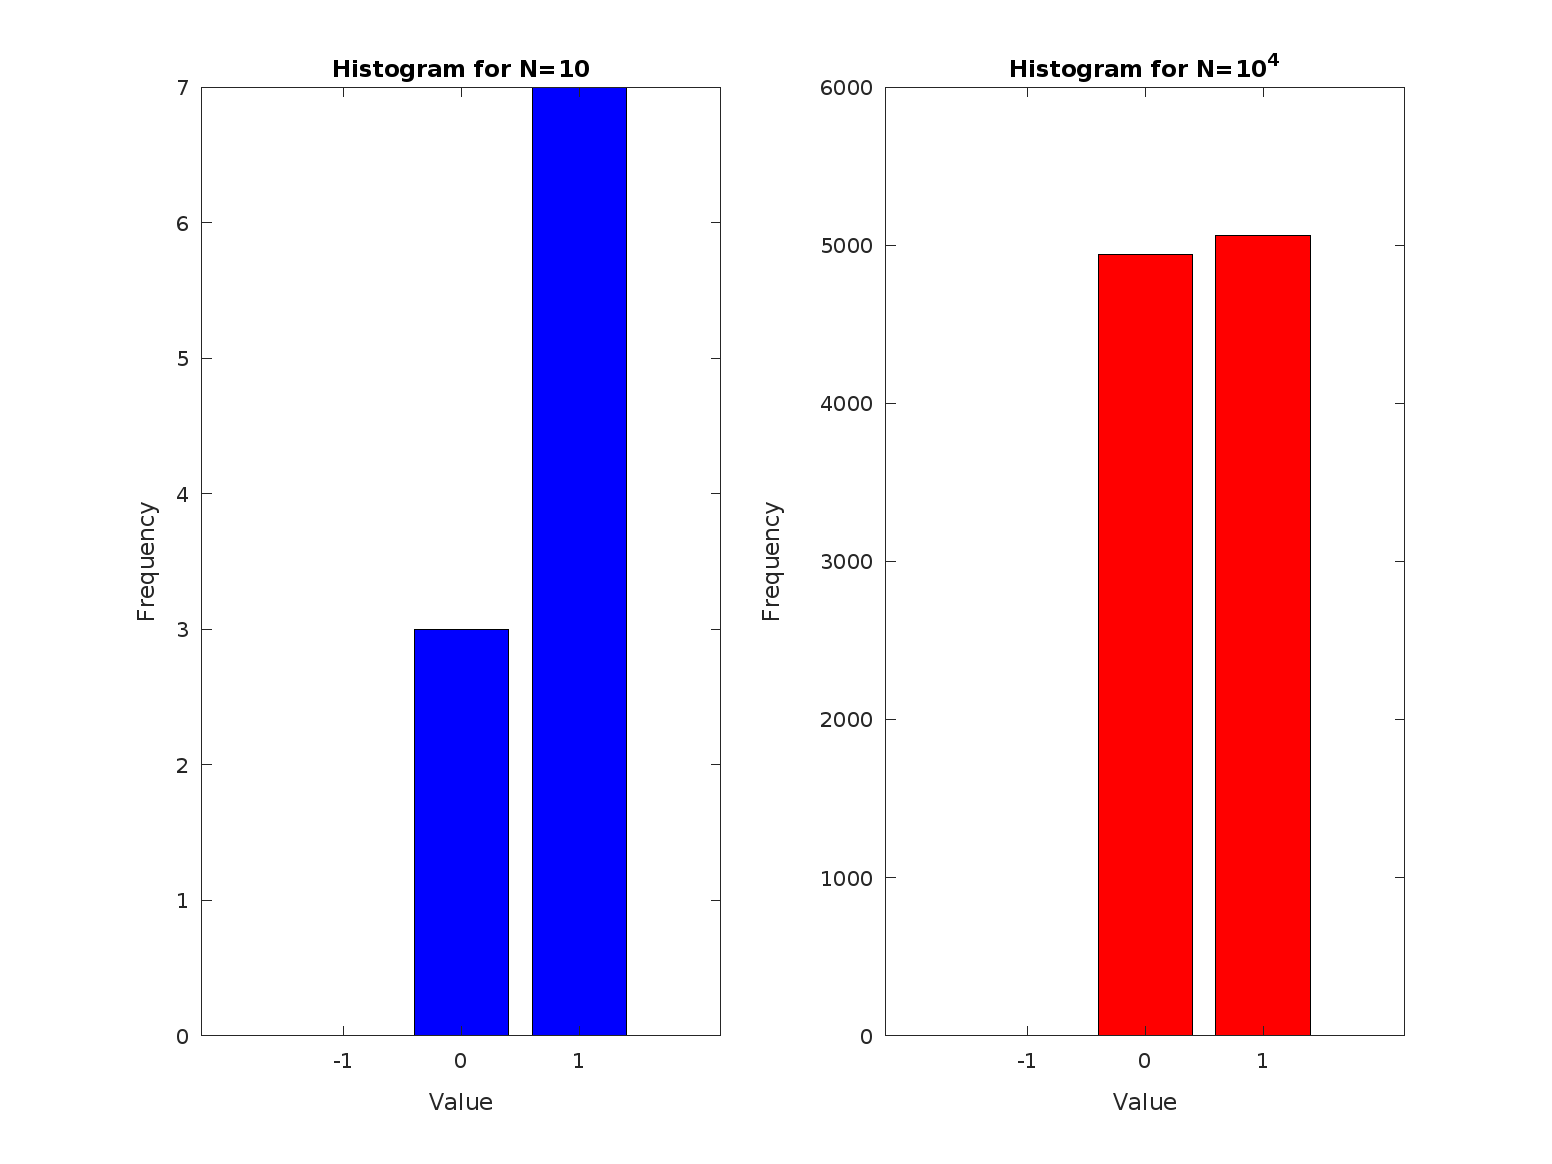
\includegraphics[width=0.8\textwidth]{histograms.png}\end{center}



\section*{Discussion}
The Probability Mass Function (PMF) graphically depicted represents a theoretically ideal distribution of our random variable \(X\), which takes the values of \(-1\) and \(1\) each with a probability of \(0.5\). Mathematically, this is expressed as \( P(X = -1) = 0.5 \) and \( P(X = 1) = 0.5 \).
\newline\newline
In comparison, the histograms generated from the MATLAB program for \(N=10\) and \(N=10^4\) illustrate empirical distributions derived from finite sets of randomly generated data. While the histogram for \(N=10\) exhibits noticeable deviations from the ideal PMF—due to the small sample size—the histogram for \(N=10^4\) closely aligns with the theoretical expectations. This is in line with the Law of Large Numbers, which states that as the size of a sample drawn from a distribution increases, the sample mean will get closer to the population mean. Mathematically, this is expressed as:

\[
\lim_{{N \to \infty}} \frac{{\sum_{i=1}^{N} X_i}}{N} = \mu
\]
where \( \mu \) is the population mean and \( X_i \) are the individual samples.
\newline \newline
Therefore, the closer alignment of the histogram for \(N=10^4\) with the PMF confirms the robustness of the random bit generator and validates the theoretical probabilities. 

\section*{MATLAB Code}
\lstinputlisting[language=Matlab]{random_bit_generator.m}

\end{document}
